
\subsection{Scalability and Generalization}








To evaluate the generalization of \ourmodel~to different teacher models, we conduct experiments using an additional Qwen3 teacher (14B) to distill students at both the 0.6B and 1.7B scales. The results are visualized in Figure~\ref{rq3}, from which we draw the following observation:







\begin{itemize}[leftmargin=*]
\item \textbf{Obs 5: \ourmodel~consistently benefits from stronger teachers, whereas OPD suffers from the increased capacity gap.}
An interesting finding emerges when comparing teacher choices under OPD: on the 0.6B student, switching from the 4B to the 14B teacher actually \emph{degrades} average accuracy by a notable margin. This reveals that a larger student-teacher capacity gap amplifies distribution mismatch, causing uniform distillation to propagate increasingly unreliable supervision. In contrast, \ourmodel~with the 14B teacher consistently outperforms its 4B counterpart on both student scales, confirming that our step-wise reweighting effectively harnesses the richer knowledge from teachers while suppressing the harmful signals introduced by the wider gap.






\begin{figure*}[t]
\centering
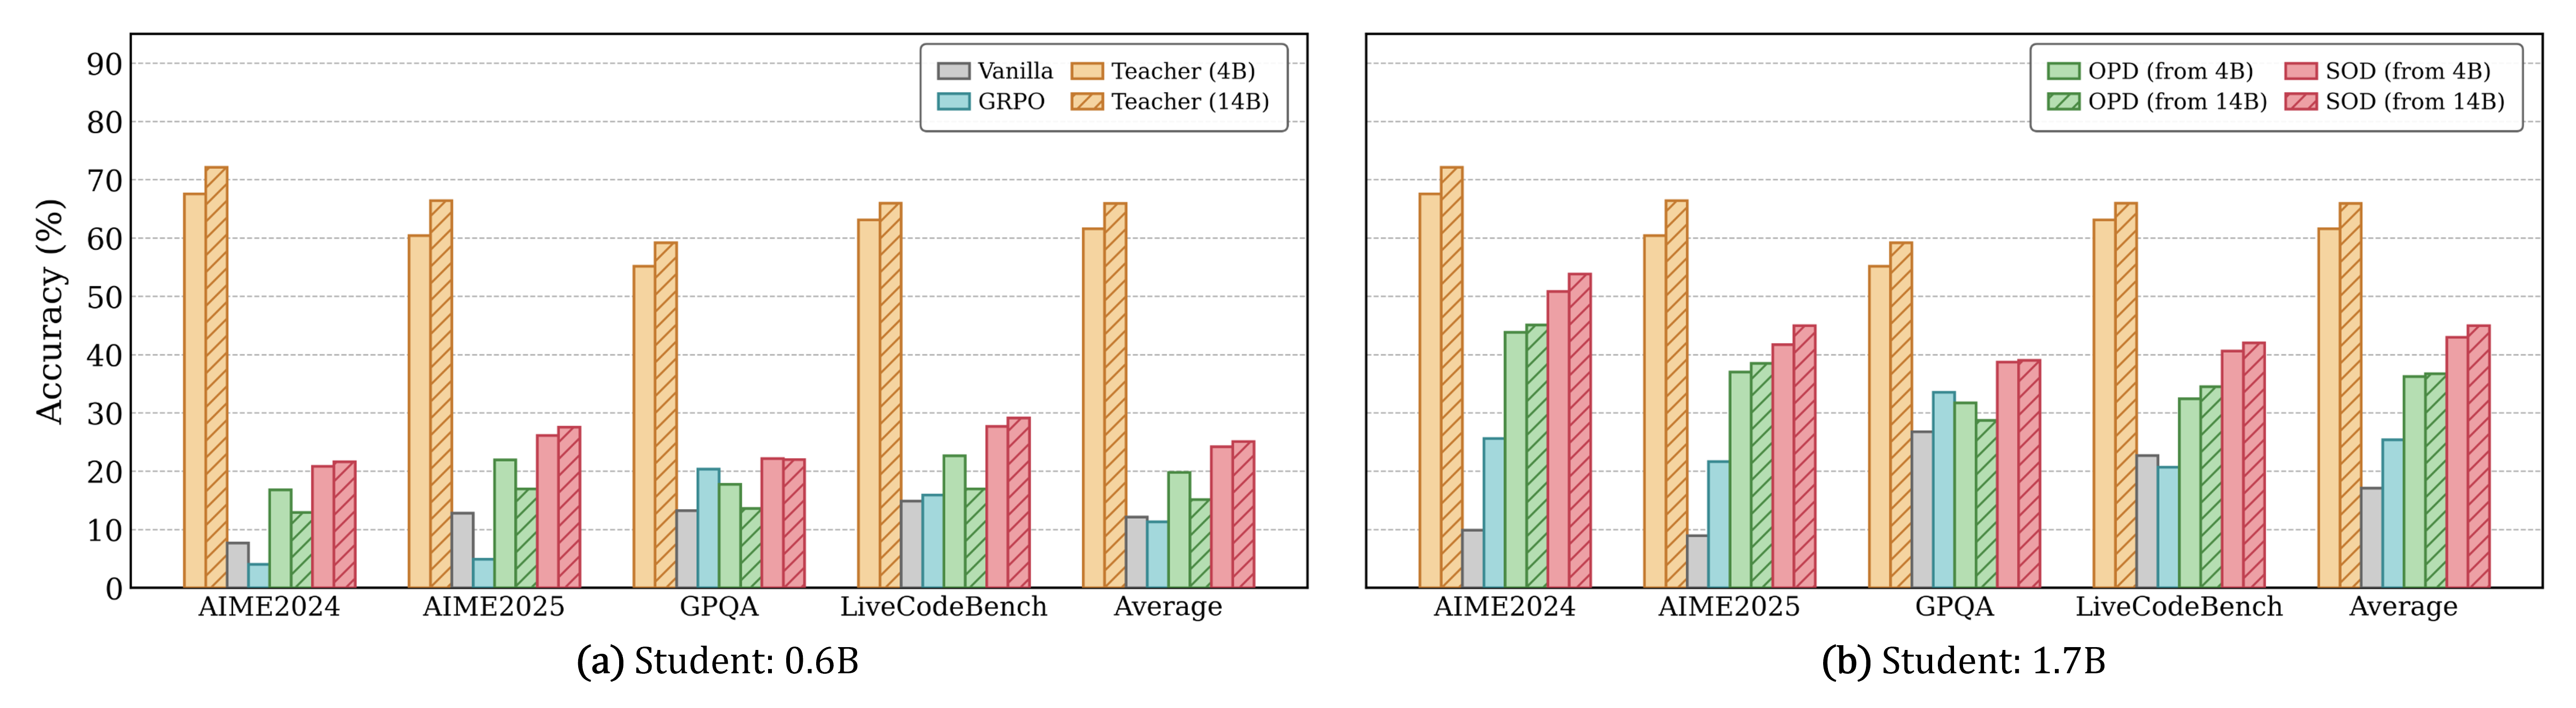
\includegraphics[width=1.0\linewidth]{pic/rq3_v9.png}
\caption{Scalability of \ourmodel~across different student-teacher configurations.}
\label{rq3}
\end{figure*}







\end{itemize}


